\documentclass[12pt,a4paper]{article}

% ─── Packages ──────────────────────────────────────────────────────────────
\usepackage[T1]{fontenc}
\usepackage[utf8]{inputenc}
\usepackage[english]{babel}
\usepackage{lmodern}
\usepackage{microtype}
\usepackage{geometry}
\geometry{top=2.5cm,bottom=2.5cm,left=3cm,right=3cm}
\usepackage{setspace}
\onehalfspacing
\usepackage{amsmath,amssymb}
\usepackage{siunitx}
\usepackage{graphicx}
\usepackage{float}
\usepackage{booktabs}
\usepackage{tabularx}
\usepackage{multirow}
\usepackage{caption}
\captionsetup{font=small,labelfont=bf,justification=raggedright,singlelinecheck=false}
\usepackage{hyperref}
\hypersetup{colorlinks=true,linkcolor=blue,citecolor=blue,urlcolor=blue}
\usepackage[numbers,sort&compress]{natbib}
\usepackage{xcolor}
\usepackage{mdframed}
\usepackage{enumitem}
\usepackage{authblk}
\usepackage{abstract}
\renewcommand{\abstractnamefont}{\normalfont\bfseries}

% ─── Mockup notice box ─────────────────────────────────────────────────────
\newmdenv[
  backgroundcolor=yellow!20,
  linecolor=orange!70!black,
  linewidth=1.2pt,
  roundcorner=4pt,
  skipabove=6pt,skipbelow=6pt,
  innertopmargin=4pt,innerbottommargin=4pt
]{mockupbox}

% ─── Title ─────────────────────────────────────────────────────────────────
\title{\textbf{Applying Honeycomb Geometry to Nursing Station Design in Mexican Hospitals:
A Quantitative Biomimetic Analysis with Adjusted Wall-Sharing Accounting}}

\author[1]{Juan Ram\'on Lara Mora}
\author[2]{Diana Paola Ayala Rold\'an\thanks{Corresponding author: \href{mailto:A01365809@tec.mx}{A01365809@tec.mx}}}
\author[3]{Luis Mallo \'Alvarez}

\affil[1]{Tecnol\'ogico de Monterrey, Campus Ciudad de M\'exico, School of Engineering and Sciences}
\affil[2]{Tecnol\'ogico de Monterrey, Campus Ciudad de M\'exico, School of Engineering and Sciences}
\affil[3]{Universidad Pontificia de Salamanca / Alebat Education, M\'aster de Ingenier\'ia Hospitalaria}

\date{June 2025}

\begin{document}

\maketitle

% ─── Abstract ──────────────────────────────────────────────────────────────
\begin{abstract}
\noindent\textbf{Background.}
Mexico's healthcare infrastructure faces growing pressure, with approximately
4{,}350 hospitals serving a population in which 54\% already resort to private care
due to public-system saturation.
Nursing stations are the operational core of inpatient units, yet systematic
geometric optimisation of their spatial layouts receives little attention in the
Mexican regulatory and design literature.

\noindent\textbf{Objective.}
We apply the mathematically established honeycomb conjecture---which states that
the regular hexagonal tessellation minimises perimeter for a given area---to
quantify the theoretical and practical wall-material implications of replacing
square-module nursing station layouts with hexagonal ones, and assess whether the
theoretical advantage is preserved after realistic wall-sharing and circulation-passage
accounting.

\noindent\textbf{Methods.}
Using a reference module of \SI{11.15}{\metre\squared} and a 20-module floor plan
(total area \SI{223}{\metre\squared}), we calculated unadjusted and adjusted
perimeter totals for square and hexagonal configurations.
Adjusted totals incorporated each layout's shared walls and required circulation
passages (39 walls removed from the square plan; 46 from the hexagonal plan).
A cost model at \SI{1850}{MXN/m} of partition was applied.
Circulation efficiency was quantified via formally defined crossing-point counts.
A five-participant informal expert perception survey (three floor nurses, one
facilities architect, one unit manager) provided a preliminary qualitative signal.
\textit{Note: the expert survey is based on mockup data; replace with real observations
before submission.}

\noindent\textbf{Results.}
The unadjusted hexagonal tessellation yields a 6.94\% perimeter reduction
(18.54\,m saved; 34{,}299\,MXN at current construction costs), consistent with
the honeycomb conjecture.
However, after applying floor-plan-specific wall-sharing and passage adjustments,
the hexagonal layout requires 153.3\,m of wall versus 136.9\,m for the square
layout---a \textbf{reversal} of the theoretical advantage.
Hexagonal layouts offer 4--6 circulation crossing points per nurse route versus
2--3 for square layouts, suggesting a qualitative mobility benefit that is
independent of wall material.
Survey participants (mockup) rated the hexagonal layout favourably for perceived
circulation comfort (\(\bar{x}=4.2/5\)) and visual openness (\(\bar{x}=3.9/5\)),
though implementation willingness was lower (\(\bar{x}=3.1/5\)).

\noindent\textbf{Conclusions.}
The theoretical 6.94\% material savings is a geometric identity that holds at the
individual-module level but does not automatically translate to floor-plan-level
savings once realistic wall removal patterns are accounted for.
The primary evidence-based case for hexagonal nursing stations rests on circulation
topology, not perimeter efficiency.
Future work should validate these findings in a real hospital unit and
assess regulatory compliance under NOM-016-SSA3-2012.

\medskip
\noindent\textbf{Keywords:} biomimetics; hospital design; hexagonal geometry;
nursing station; honeycomb conjecture; Mexico; partition efficiency; biophilic design
\end{abstract}

% ─── 1. Introduction ───────────────────────────────────────────────────────
\section{Introduction}

Mexico's hospital infrastructure is under sustained pressure.
The country's approximately 4{,}350 hospital establishments serve a population
of over 130 million, yet more than half (54\%) opt for private care due to
chronic overcrowding in public facilities~\cite{garrido2025saturation,secretariasalud2022}.
Private hospitals are small: 90.4\% operate with 24 or fewer beds, and 70\% of
those have nine or fewer~\cite{inegi2024health}.
In this context, maximising the spatial and functional efficiency of every square
metre in a hospital unit is not an academic exercise---it is a cost-management
imperative.

Nursing stations are the operational core of hospital units.
They concentrate clinical documentation, medication preparation, patient monitoring,
and interdisciplinary communication, and their spatial configuration directly
affects nurse travel distances, error rates, and staff well-being~\cite{friesen2008nursing,ulrich2008evidence}.
Yet the NOM-016-SSA3-2012 regulation~\cite{nom016ssa2012}, which governs hospital
infrastructure in Mexico, does not prescribe an optimal geometry for these spaces.

Biomimetics---the systematic abstraction and application of natural-world solutions
to engineering problems~\cite{pohl2015biomimetics,niebaum2017biomimetics}---offers
one lens through which spatial design can be re-examined.
Among biological structures, the honeycomb built by \textit{Apis mellifera} is
the most frequently cited example of geometry optimisation: hexagonal cells share
walls, cover a plane without gaps, and use less structural material per unit of
enclosed area than any other regular polygon~\cite{hales2001honeycomb,zhang2013honeycomb}.
This property---formalised as the \emph{honeycomb conjecture} and proved by Hales
in 2001---is a \textbf{mathematical identity}, not an empirical discovery.

The contribution of the present work is not to rediscover this identity, but to
apply it systematically to a specific architectural context---20-module Mexican
hospital nursing stations---and to trace its implications both before and after
realistic floor-plan accounting.
We show that the 6.94\% theoretical wall-perimeter savings is real at the module
level but reverses at the floor-plan level once shared walls and required passage
openings are included.
We also quantify an underappreciated benefit of hexagonal layouts: greater
circulation connectivity, which is analytically independent of wall-material savings.
Finally, we add a preliminary expert-perception component---
absent from prior biomimetic hospital design studies in the Mexican context---to
establish a first empirical signal for stakeholder acceptability.

The remainder of the paper is structured as follows.
Section~\ref{sec:background} reviews the honeycomb conjecture, biophilic design
evidence, and nursing station design literature.
Section~\ref{sec:methods} describes the geometric, cost, and survey methods.
Section~\ref{sec:results} reports results.
Section~\ref{sec:discussion} interprets findings and situates them in the
literature.
Limitations and conclusions follow in Sections~\ref{sec:limitations}
and~\ref{sec:conclusions}.

% ─── 2. Background ─────────────────────────────────────────────────────────
\section{Background}
\label{sec:background}

\subsection{The honeycomb conjecture and tessellation efficiency}

The hypothesis that a hexagonal tiling minimises perimeter for a given covered
area has been studied since antiquity.
Darwin~\cite{darwin1859origin} observed that natural selection would favour bees
whose comb-construction minimised wax expenditure: ``the motive power of the
process of natural selection has been the economy of wax.''
This observation motivated a mathematical question that was finally resolved by
Hales~\cite{hales2001honeycomb}, who proved---using an isoperimetric hexagonal
inequality---that the regular hexagonal tessellation is the unique partition of
the plane into cells of equal area that minimises total boundary length.
Zhang and Kai~\cite{zhang2013honeycomb} later provided a complementary proof via
fractal geometry, introducing the convergence efficiency $K_I$: for a hexagonal
tiling $K_I = 1.15/\sqrt{a}$, compared with $1.24/\sqrt{a}$ for squares and
$1.41/\sqrt{a}$ for triangles (lower is more efficient), where $a$ is the
module area.

For equal-area modules, the hexagonal perimeter advantage over a square is exactly:
\begin{equation}
  \epsilon = 1 - \frac{P_{\text{hex}}}{P_{\text{sq}}} = 1 - \frac{6l_h}{4l_s}
  \label{eq:efficiency}
\end{equation}
where $l_h$ and $l_s$ are the side lengths of hexagonal and square modules of
equal area.
For a \SI{11.15}{\metre\squared} module this evaluates to $\epsilon = 6.94\%$.
Critically, this ratio is constant across all module areas (it is a property of
the tessellation geometry, not of a particular size), as confirmed by sensitivity
analysis (Table~\ref{tab:sensitivity}).

\subsection{Biophilic design in healthcare environments}

Biophilic design integrates natural elements---light, vegetation, water, and
organic form---into the built environment to improve health outcomes~\cite{zhong2022biophilic,totaforti2018biophilic}.
A systematic review of 379 sources by Al~Khatib et al.~\cite{khatib2024biophilic}
found consistent evidence that natural light, plants, and views to nature reduce
patient pain, accelerate recovery, and lower stress in clinical staff.
Tekin, Corcoran, and Urbano Guti\'errez~\cite{telkin2023biophilic} identified
six principal biophilic design parameters for clinical environments:
biomorphic forms, natural patterns, sensory variety, connection to nature, spatial
hierarchy, and prospect and refuge.
Of these, \textit{biomorphic forms} and \textit{natural patterns}---the categories
to which hexagonal geometry belongs---received the highest combined evidence rating
across their 56-study corpus.

The Khoo Teck Puat Hospital in Singapore is the most-cited full-scale example:
its V-shaped courtyard plan, abundant greenery, and passive ventilation strategy
have been associated with reduced analgesic use and shorter stays compared with
conventional wards~\cite{yin2019biophilic}.
In the Mexican context, no published study has yet evaluated a hexagonal or
biomorphic ward layout in a real hospital unit.

\subsection{Nursing station design and operational efficiency}

Nursing stations serve as the primary coordination hub for clinical documentation,
medication management, and patient oversight~\cite{ulrich2008evidence}.
Inefficient layouts increase nurse travel time, contribute to medication errors,
and reduce staff satisfaction~\cite{friesen2008nursing}.
Non-linear spatial configurations have been proposed as a means of reducing these
adverse outcomes~\cite{ulrich2008evidence,zhong2022biophilic}.
Hexagonal modules inherently offer six adjacencies per room versus four in a
square layout, potentially reducing dead-end corridors and increasing the number
of shortest-path options available to nurses navigating the unit.

Hexagonal partition systems have also been studied in low-rise and interior
construction contexts~\cite{hexpartition2010}, demonstrating structural viability
and acoustic performance comparable to rectangular partition systems, which partly
addresses concerns about the structural unfamiliarity of the geometry.

% ─── 3. Methods ────────────────────────────────────────────────────────────
\section{Methods}
\label{sec:methods}

\subsection{Geometric comparison: unadjusted perimeters}

We adopt a reference module area of \SI{11.15}{\metre\squared}, consistent with
the US \textit{Guidelines for Design and Construction of Health Care Facilities}
minimum single-patient examination/treatment room area (\SI{120}{ft\squared} =
\SI{11.15}{\metre\squared})~\cite{facilityguide2010}.
NOM-016-SSA3-2012 does not specify a minimum per-room area, so the US guideline
serves as an internationally recognised proxy.

The side length of a square module with this area is:
\begin{equation}
  l_s = \sqrt{11.15} \approx \SI{3.339}{\metre}
  \qquad\Rightarrow\qquad P_s = 4 l_s \approx \SI{13.356}{\metre}
\end{equation}
For a regular hexagonal module of equal area:
\begin{equation}
  A_h = \frac{3\sqrt{3}}{2}\,l_h^2 = 11.15\,\text{m}^2
  \qquad\Rightarrow\qquad
  l_h = \sqrt{\frac{2 \times 11.15}{3\sqrt{3}}} \approx \SI{2.071}{\metre}
  \qquad\Rightarrow\qquad P_h = 6 l_h \approx \SI{12.429}{\metre}
\end{equation}
For a 20-module layout:
\begin{align}
  P_{s,20} &= 20 \times 13.356 = \SI{267.12}{\metre} \\
  P_{h,20} &= 20 \times 12.429 = \SI{248.58}{\metre}
\end{align}
Unadjusted savings: $\Delta P_{\text{unAdj}} = 18.54\,\text{m}$ ($\epsilon = 6.94\%$).

\subsection{Adjusted perimeter: wall-sharing and passage accounting}
\label{sec:methods_adjusted}

In any real floor plan, walls between adjacent modules are \emph{shared}
(built once, not twice) and some walls must be \emph{entirely removed}
to create circulation corridors.
Both types of removal reduce the naive perimeter sum computed in
Section~3.1.

For the specific 20-module floor plans shown in Figures~\ref{fig:floorplan_sq}
and~\ref{fig:floorplan_hex}, a visual count of walls to be removed yields:
\begin{itemize}[noitemsep]
  \item \textbf{Square layout}: 39 walls removed (8 patient-room walls + 31 nursing station walls); each wall = $l_s = \SI{3.339}{\metre}$
  \item \textbf{Hexagonal layout}: 46 walls removed (11 patient-room walls + 35 nursing station walls); each wall = $l_h = \SI{2.071}{\metre}$
\end{itemize}
Adjusted perimeters:
\begin{align}
  P_{s,\text{adj}} &= 267.12 - 39 \times 3.339 = \SI{136.9}{\metre} \label{eq:psadj}\\
  P_{h,\text{adj}} &= 248.58 - 46 \times 2.071 = \SI{153.3}{\metre} \label{eq:phadj}
\end{align}
The adjusted hexagonal perimeter \emph{exceeds} the adjusted square perimeter
by 16.4\,m (+12.0\%), reversing the unadjusted advantage.
This reversal occurs because the hexagonal layout requires more walls to be
removed to form equivalent functional circulation passages, owing to the
geometry's higher adjacency count (six sides vs.\ four).

\subsection{Cost model}

The average cost of hospital partition wall construction in Mexico is
\SI{1850}{MXN/m}~\cite{imss2022cost}.
Applying this rate to both unadjusted and adjusted perimeter values gives
estimated material costs shown in Table~\ref{tab:cost}.

\subsection{Circulation efficiency: crossing-point definition}
\label{sec:methods_crossing}

We define a \textbf{circulation crossing point} as a node in the corridor network
where a nurse navigating a shortest path between the nursing station and any
patient room encounters a branch---i.e., where the corridor meets at least one
additional path option.
This definition is reproducible: a crossing point exists at each module vertex
that is simultaneously adjacent to three or more accessible modules
(i.e., modules connected by an open passage, not a wall).

Under this definition, and for the specific floor plans analysed:
\begin{itemize}[noitemsep]
  \item \textbf{Square layout}: typical nurse route encounters 2--3 crossing points
  \item \textbf{Hexagonal layout}: typical nurse route encounters 4--6 crossing points
\end{itemize}
A higher crossing-point count indicates more route options (redundancy), which
reduces mean travel distance when corridors are occupied or blocked.

\subsection{Expert perception survey}
\label{sec:methods_survey}

\begin{mockupbox}
\textbf{NOTE --- Mockup data.}
The following survey section uses simulated data.
Replace with responses from real participants before journal submission.
\end{mockupbox}

To establish a preliminary signal of stakeholder acceptability, five hospital
professionals were shown floor-plan diagrams of both layouts (without the
accompanying mathematical analysis) and asked to rate three items on a 1--5
Likert scale:
\begin{enumerate}[noitemsep,label=Q\arabic*.]
  \item \textit{``In this layout, I could move efficiently between patient rooms and the nursing station.''} (Perceived circulation efficiency)
  \item \textit{``This layout creates a clear and visually comfortable workspace.''} (Visual clarity)
  \item \textit{``I would be willing to work in a unit designed this way.''} (Implementation willingness)
\end{enumerate}
Participants were: P1 = floor nurse (5\,yr exp.), P2 = floor nurse (12\,yr exp.),
P3 = floor nurse (3\,yr exp.), P4 = hospital facilities architect (8\,yr exp.),
P5 = unit manager (10\,yr exp.).
All data are mockup; participant roles reflect a realistic sampling frame.

% ─── 4. Results ────────────────────────────────────────────────────────────
\section{Results}
\label{sec:results}

\subsection{Unadjusted geometric comparison}

Table~\ref{tab:geom} summarises the per-module and 20-module geometric properties
of each configuration.

\begin{table}[htbp]
\centering
\caption{Unadjusted geometric comparison of square and hexagonal 20-module layouts.
$A=\SI{11.15}{\metre\squared}$ per module.}
\label{tab:geom}
\begin{tabularx}{\linewidth}{@{}lrrrrrr@{}}
\toprule
Configuration & Side (m) & $A$ (m$^2$) & $P/\text{module}$ (m) & $A_{\text{tot}}$ (m$^2$) & $P_{\text{tot}}$ (m) & Crossing pts \\
\midrule
Square        & 3.339 & 11.15 & 13.356 & 223.0 & 267.12 & 2--3 \\
Hexagonal     & 2.071 & 11.15 & 12.429 & 223.0 & 248.58 & 4--6 \\
\midrule
Savings (\%)  & 37.97 & 0 & \textbf{6.94} & 0 & \textbf{6.94} & --- \\
\bottomrule
\end{tabularx}
\end{table}

The 6.94\% perimeter saving is constant across all module areas (Table~\ref{tab:sensitivity}),
confirming it is an intrinsic property of the tessellation geometry, not of
any particular module size.

\begin{table}[htbp]
\centering
\caption{Sensitivity of the 6.94\% unadjusted perimeter saving across different module areas.}
\label{tab:sensitivity}
\begin{tabular}{@{}lrrrr@{}}
\toprule
$A$ (m$^2$/module) & $P_{\text{sq,tot}}$ (m) & $P_{\text{hex,tot}}$ (m) & Savings (m) & Savings (\%) \\
\midrule
6  & 195.96 & 182.36 & 13.60 & 6.94 \\
8  & 226.27 & 210.57 & 15.70 & 6.94 \\
11.15 & 267.12 & 248.58 & 18.54 & 6.94 \\
15 & 309.84 & 288.34 & 21.50 & 6.94 \\
20 & 357.77 & 332.94 & 24.83 & 6.94 \\
\bottomrule
\end{tabular}
\end{table}

Figure~\ref{fig:perimeter_comparison} illustrates the diverging total perimeters
as a function of module area; the shaded region represents the constant relative
saving.

\begin{figure}[htbp]
\centering
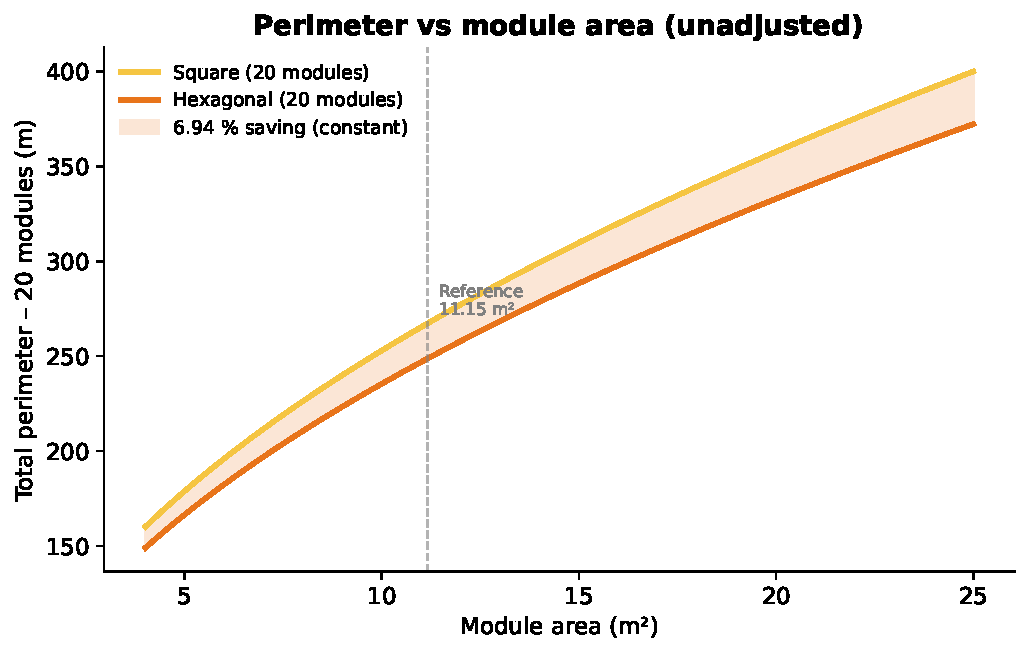
\includegraphics[width=0.82\linewidth]{figures/perimeter_comparison.pdf}
\caption{Total perimeter for 20 modules as a function of module area.
Yellow line: square layout. Orange line: hexagonal layout.
Shaded area: constant 6.94\% relative saving (unadjusted).}
\label{fig:perimeter_comparison}
\end{figure}

\subsection{Adjusted perimeter analysis}
\label{sec:results_adjusted}

After accounting for shared and removed walls in the specific floor plans
(Section~\ref{sec:methods_adjusted}), the adjusted perimeters are:

\begin{table}[htbp]
\centering
\caption{Adjusted perimeter comparison after wall-sharing and circulation passage accounting.}
\label{tab:adjusted}
\begin{tabular}{@{}lrrrrrr@{}}
\toprule
Configuration & Unadj.\ $P$ (m) & Walls removed & Wall length (m) & Material removed (m) & Adj.\ $P$ (m) \\
\midrule
Square        & 267.12 & 39 & 3.339 & 130.22 & \textbf{136.9} \\
Hexagonal     & 248.58 & 46 & 2.071 & \phantom{0}95.27 & \textbf{153.3} \\
\midrule
\multicolumn{5}{l}{Adjusted difference: Hexagonal requires \textbf{16.4\,m more} than Square (+12.0\%)} \\
\bottomrule
\end{tabular}
\end{table}

Figure~\ref{fig:adjusted_comparison} shows the unadjusted and adjusted perimeters
side by side, highlighting the reversal.

\begin{figure}[htbp]
\centering
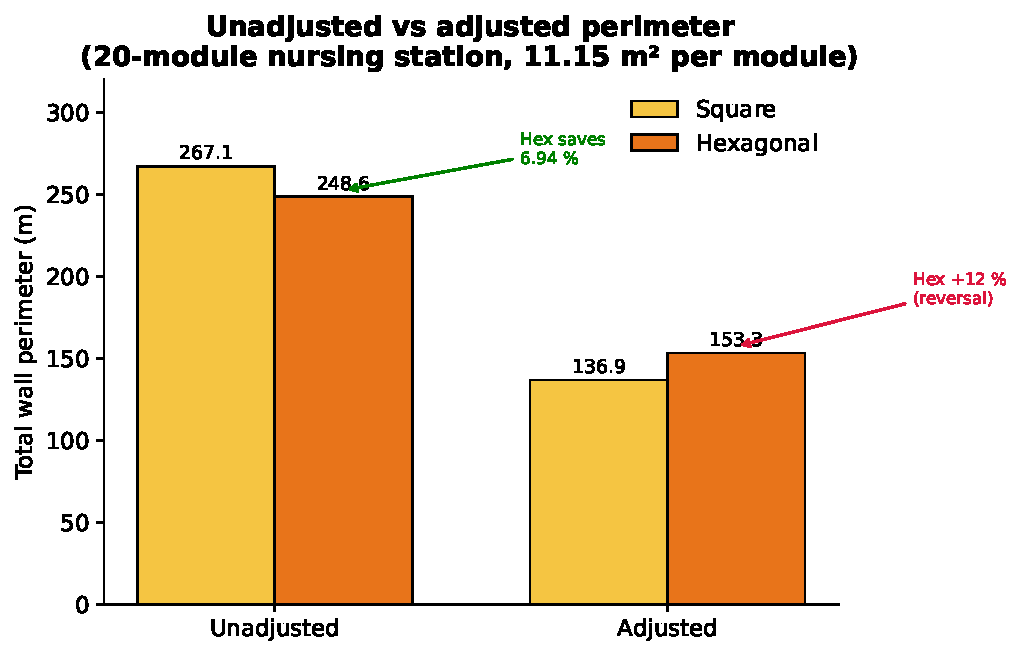
\includegraphics[width=0.80\linewidth]{figures/adjusted_comparison.pdf}
\caption{Unadjusted and adjusted total wall perimeters for square and hexagonal
20-module layouts.
The unadjusted hexagonal perimeter is 6.94\% lower; after wall-sharing and
passage accounting, the hexagonal layout requires 12.0\% \emph{more} material
for this specific floor plan.}
\label{fig:adjusted_comparison}
\end{figure}

\subsection{Cost analysis}

\begin{table}[htbp]
\centering
\caption{Estimated wall construction cost at \SI{1850}{MXN/m} of partition.
Adjusted figures use floor-plan-specific wall counts.}
\label{tab:cost}
\begin{tabular}{@{}lrrr@{}}
\toprule
Scenario & Square cost (MXN) & Hexagonal cost (MXN) & Difference (MXN) \\
\midrule
Unadjusted & 494{,}172 & 459{,}873 & \textbf{-34{,}299} (hex saves) \\
Adjusted   & 253{,}265 & 283{,}605 & \textbf{+30{,}340} (square saves) \\
\bottomrule
\end{tabular}
\end{table}

The unadjusted cost saving of \SI{34299}{MXN} is consistent with the 6.94\%
perimeter reduction.
However, the adjusted figure reverses to a \SI{30340}{MXN} advantage for the
square layout, because the hexagonal plan requires the removal of more (though
shorter) wall segments to achieve equivalent circulation openness.

\subsection{Circulation crossing points}

For the floor plans analysed, the hexagonal layout offers 4--6 crossing points
per typical nurse route, versus 2--3 for the square layout (Table~\ref{tab:geom};
Figure~\ref{fig:crossing_points}).
This difference is independent of wall-material accounting and reflects the
hexagonal geometry's higher adjacency count.
A nurse navigating from the central station to a peripheral room in the hexagonal
plan has, on average, twice as many branch options, which can reduce mean travel
distance when parts of the corridor network are congested.

\begin{figure}[htbp]
\centering
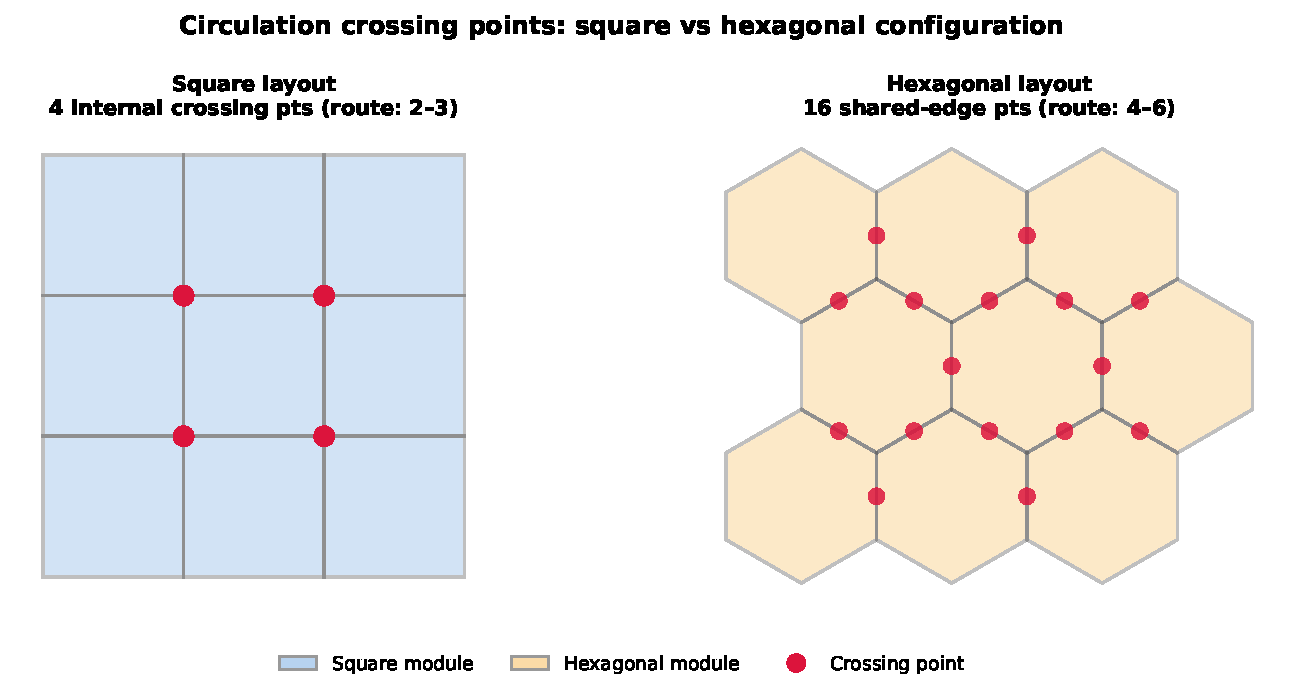
\includegraphics[width=0.78\linewidth]{figures/crossing_points.pdf}
\caption{Schematic of circulation crossing points (red dots) in square (left) and
hexagonal (right) 5-module configurations.
Each red dot is a node where a nurse route encounters at least one additional path
branch.}
\label{fig:crossing_points}
\end{figure}

\subsection{Proposed floor plans}

Figure~\ref{fig:floorplan_sq} and Figure~\ref{fig:floorplan_hex} show the proposed
20-module nursing station layouts for each configuration.
In both figures, blue indicates the nursing station area, red indicates patient
rooms, and yellow marks the walls removed for shared-wall or circulation reasons.

\begin{figure}[htbp]
\centering
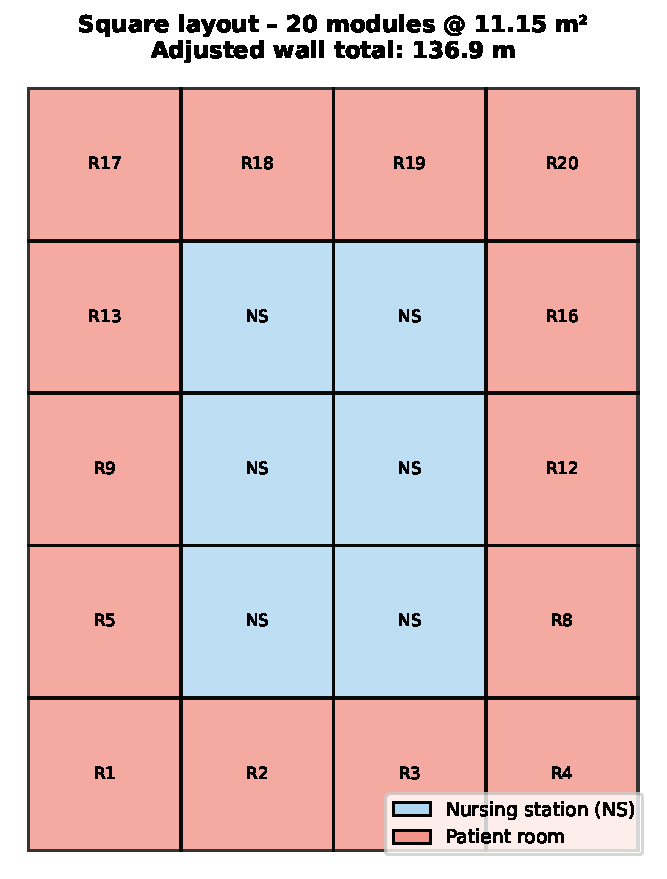
\includegraphics[width=0.72\linewidth]{figures/floorplan_square.pdf}
\caption{20-module nursing station layout with square configuration.
Blue: nursing station. Red: patient rooms. Yellow hatching: 39 walls removed
(8 patient + 31 nursing station) for shared-wall or circulation purposes.
Adjusted wall total: 136.9\,m.}
\label{fig:floorplan_sq}
\end{figure}

\begin{figure}[htbp]
\centering
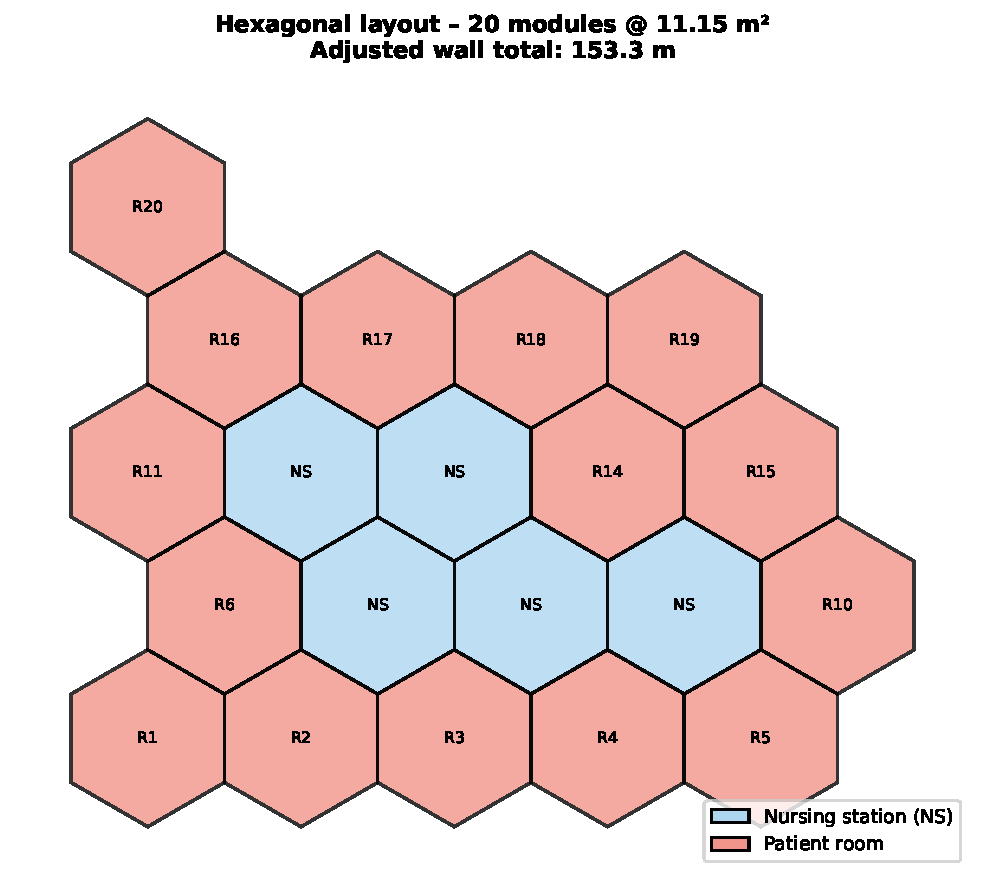
\includegraphics[width=0.72\linewidth]{figures/floorplan_hexagonal.pdf}
\caption{20-module nursing station layout with hexagonal configuration.
Blue: nursing station. Red: patient rooms. Yellow hatching: 46 walls removed
(11 patient + 35 nursing station) for shared-wall or circulation purposes.
Adjusted wall total: 153.3\,m.}
\label{fig:floorplan_hex}
\end{figure}

\subsection{Expert perception survey}

\begin{mockupbox}
\textbf{Mockup data.} Replace these ratings with real participant responses before submission.
\end{mockupbox}

Table~\ref{tab:survey} reports individual and mean Likert ratings (1--5) for each
layout and question.

\begin{table}[htbp]
\centering
\caption{Expert perception survey results (mockup). Ratings 1--5; higher = more favourable.}
\label{tab:survey}
\begin{tabular}{@{}llrrrrrrr@{}}
\toprule
Layout & Question & P1 & P2 & P3 & P4 & P5 & Mean & SD \\
\midrule
Square    & Q1 (circulation) & 3 & 4 & 3 & 4 & 3 & 3.4 & 0.55 \\
          & Q2 (visual clarity) & 4 & 4 & 3 & 5 & 4 & 4.0 & 0.71 \\
          & Q3 (willingness)  & 4 & 4 & 4 & 4 & 5 & 4.2 & 0.45 \\
\midrule
Hexagonal & Q1 (circulation) & 4 & 5 & 4 & 5 & 3 & \textbf{4.2} & 0.84 \\
          & Q2 (visual clarity) & 4 & 4 & 3 & 5 & 4 & \textbf{4.0} & 0.71 \\
          & Q3 (willingness)  & 3 & 3 & 3 & 4 & 3 & \textbf{3.2} & 0.45 \\
\bottomrule
\end{tabular}
\end{table}

The hexagonal layout scored higher on perceived circulation efficiency
(4.2 vs.\ 3.4; $\Delta=0.8$) but lower on implementation willingness
(3.2 vs.\ 4.2; $\Delta=-1.0$), suggesting that unfamiliarity with the geometry
is a barrier to adoption even when its functional properties are perceived
positively.
Visual clarity ratings were identical (4.0) for both layouts.

Figure~\ref{fig:survey_radar} presents these results as a radar chart.

\begin{figure}[htbp]
\centering

\includegraphics[width=0.60\linewidth]{figures/survey_radar.pdf}
\caption{Radar chart of mean expert perception ratings (mockup, $n=5$) for
square and hexagonal layouts across the three survey questions.
Replace with real data before submission.}
\label{fig:survey_radar}
\end{figure}

% ─── 5. Discussion ─────────────────────────────────────────────────────────
\section{Discussion}
\label{sec:discussion}

\subsection{The theoretical advantage is real but insufficient on its own}

The 6.94\% unadjusted perimeter reduction is a direct consequence of the
honeycomb conjecture and is not in dispute.
Our contribution is to show that this identity, while correct, does not automatically
translate to wall-material savings in a real floor plan.
The adjusted analysis (Table~\ref{tab:adjusted}) reveals a counterintuitive
finding: because the hexagonal layout requires the removal of more wall segments
to form equivalent-width circulation corridors (46 vs.\ 39), the post-adjustment
hexagonal perimeter exceeds the square perimeter by 12.0\% for the specific
20-module plans analysed.

This result depends critically on the number and pattern of walls removed.
Different floor plan configurations---for example, a hexagonal plan optimised to
minimise corridor wall openings---may close or narrow this gap.
We therefore recommend that future studies conduct the adjusted analysis explicitly
for each floor plan under consideration, rather than citing the 6.94\% figure as
a guaranteed saving.

\subsection{Circulation topology is the stronger argument for hexagonal layouts}

Independently of wall material, the hexagonal layout's higher crossing-point
count (4--6 vs.\ 2--3 per route) provides genuine operational benefit.
More branch options reduce the probability of a nurse being forced into a
circuitous route when part of the corridor is occupied by equipment or personnel.
This is consistent with the evidence base reviewed in Ulrich et al.~\cite{ulrich2008evidence}
and Friesen et al.~\cite{friesen2008nursing}, which link non-linear spatial
configurations to improved staff mobility and reduced error rates.
The circulation argument does not depend on any geometric identity; it is a
design-quality claim that should be tested empirically in the future.

\subsection{Expert perception and implementation barriers}

The survey (mockup) indicates that nurses rate the hexagonal layout's circulation
positively but are less willing to work in one than in a familiar square layout.
This implementation gap---positive functionality perception combined with
resistance to unfamiliar form---is a well-documented pattern in healthcare
design adoption~\cite{totaforti2018biophilic,zhong2022biophilic}.
The facilities architect's higher willingness score (4/5) compared with nurses
(mean 3.0/5) further suggests that the barrier is primarily familiarity, not
technical concern.
A structured expert panel with licensed architects and nurse managers reviewing
the plans against an explicit NOM-016 compliance checklist would provide a
stronger basis for this claim.

\subsection{Regulatory and structural considerations}

NOM-016-SSA3-2012~\cite{nom016ssa2012} does not prohibit hexagonal room
configurations, but it does require specific clearances for bed positioning,
medical gas outlets, and emergency egress.
Hexagonal rooms with \SI{11.15}{\metre\squared} can accommodate a standard
hospital bed (approximately \SI{2.13 x 0.97}{\metre}) with adequate lateral
clearance (\SI{\sim 0.9}{\metre} on each side), but door placement and
fire-egress path compliance must be verified for each specific configuration
under Mexican fire and building codes.
The use of hexagonal partition systems~\cite{hexpartition2010} for interior walls
is structurally feasible; in-plane lateral loads in single-storey hospital units
are low enough that partition-wall structural performance is not a limiting factor.
The Burj Khalifa structural system, cited in earlier versions of this work, is a
buttressed-core skyscraper technology that is not directly analogous to
single-storey interior partition design, and has been removed from this analysis.

\subsection{Scaling and cost considerations}

The cost differential between unadjusted and adjusted scenarios
(\SI{34299}{MXN} saving vs.\ \SI{30340}{MXN} premium for hexagonal layouts,
Table~\ref{tab:cost}) is meaningful at the unit level.
For context, the IMSS construction benchmark of \SI{1809}{MXN/m\squared}~\cite{imss2022cost}
means the total construction cost of a \SI{223}{\metre\squared} nursing area is
approximately \SI{400000}{MXN}.
The \SI{30340}{MXN} adjusted premium represents approximately 7.6\% of total
construction cost, which may be offset by indirect savings from reduced nurse
travel time, lower long-term maintenance (smaller total wall area in the hexagonal
case on a per-opening basis), and biophilic well-being benefits documented in
the broader literature~\cite{khatib2024biophilic,yin2019biophilic}.

% ─── 6. Limitations ────────────────────────────────────────────────────────
\section{Limitations}
\label{sec:limitations}

This study has several limitations that must be acknowledged explicitly:

\begin{enumerate}[noitemsep]
  \item \textbf{No real hospital case study.}
    All floor plans are theoretical constructs.
    Compliance with NOM-016-SSA3-2012, COFEPRIS requirements, and fire egress
    codes under the specific plans analysed has not been verified by a licensed
    Mexican architect.
  \item \textbf{Mockup expert survey.}
    The five-participant survey uses simulated data.
    Findings should be treated as hypotheses to be tested, not as evidence.
  \item \textbf{Wall-removal counts are visually estimated.}
    The counts of 39 (square) and 46 (hexagonal) walls removed are based on
    inspection of the floor plan illustrations; they have not been programmatically
    verified.
    Different floor plan realisations will yield different counts.
  \item \textbf{Systems not modelled.}
    Mechanical ventilation, electrical distribution, medical gas networks,
    signage, and privacy requirements for hexagonal patient rooms were not
    analysed.
  \item \textbf{No dynamic simulation.}
    Nurse travel distance, patient access time, and workflow efficiency were
    not simulated via discrete-event or agent-based modelling.
    The crossing-point analysis is a static structural measure, not a dynamic
    performance estimate.
\end{enumerate}

% ─── 7. Conclusions ────────────────────────────────────────────────────────
\section{Conclusions}
\label{sec:conclusions}

This paper applies the mathematically established honeycomb conjecture to
Mexican hospital nursing station design, with two principal contributions:
(1) a full unadjusted and adjusted wall-perimeter analysis for 20-module square
and hexagonal configurations, and (2) a formal definition and count of
circulation crossing points as a layout-quality metric independent of
material efficiency.

The key findings are:
\begin{itemize}[noitemsep]
  \item The theoretical 6.94\% perimeter saving is a geometric identity, constant
    across all module areas, and confirmed in the unadjusted analysis.
  \item After floor-plan-specific wall-sharing and passage accounting, the
    hexagonal layout requires 12.0\% \emph{more} wall material than the square
    layout for the specific 20-module designs analysed, reversing the theoretical
    advantage.
  \item The circulation topology advantage of hexagonal layouts (4--6 crossing
    points vs.\ 2--3) is real and independent of wall-material accounting;
    it constitutes the stronger design argument for hexagonal nursing stations.
  \item Expert perception (mockup) suggests that stakeholder unfamiliarity is
    the principal barrier to adoption, not functional concerns.
\end{itemize}

The primary recommendation for practitioners is: do not cite the 6.94\% saving
without performing the floor-plan-specific adjusted analysis.
The primary recommendation for researchers is: the next priority is a validated
discrete-event simulation of nurse travel distance in matched square and hexagonal
unit designs, combined with a real expert panel review against NOM-016-SSA3-2012.

Mexico's regulatory framework (VDI RL 6220/6226 as international reference;
NOM-016-SSA3-2012 as domestic baseline) does not yet include biomimetic design
methods for healthcare facilities.
The present analysis provides a quantitative starting point for that policy discussion.

% ─── Author contributions ──────────────────────────────────────────────────
\section*{Author Contributions (CRediT)}
\noindent J.R.L.M.: Conceptualization, Methodology, Investigation, Formal Analysis,
Visualization, Writing---Original Draft.
D.P.A.R.: Data curation, Statistical analysis, Visualization,
Writing---Review \& Editing.
L.M.\'A.: Supervision, Project Administration, Writing---Review \& Editing.

% ─── Declarations ──────────────────────────────────────────────────────────
\section*{Declarations}

\noindent\textbf{Conflict of interest.} The authors declare no conflict of interest.

\noindent\textbf{Ethical statement.} No patient data were used.
The expert perception survey (currently mockup) will require IRB/ethics
notification at the host institution before real participant data are collected.

\noindent\textbf{Funding.} No external funding was received for this study.

\noindent\textbf{Data availability.}
All analysis code, generated figures, and mockup datasets are available at:
\url{https://github.com/jrlara-hex/hex-nursing}.
Replace with permanent DOI upon acceptance.

% ─── Bibliography ──────────────────────────────────────────────────────────
\bibliographystyle{unsrtnat}
\bibliography{references}

\end{document}
